\documentclass[12pt,a4paper]{article}
\usepackage[utf8]{inputenc}
\usepackage{graphicx}
\usepackage{hyperref}
\usepackage{booktabs}
\usepackage{xcolor}
\usepackage{geometry}
\geometry{a4paper, margin=1in}
\usepackage{fancyhdr}
\usepackage{float}
\usepackage{titlesec}
\usepackage{enumitem}

% Define colors matching the official MSA branding guidelines (NFR35)
\definecolor{msanavy}{HTML}{1F3864}
\definecolor{msagold}{HTML}{8B6914}
\definecolor{lightgray}{gray}{0.95}

% Document settings
\hypersetup{
    colorlinks=true,
    linkcolor=msanavy,
    filecolor=msagold,      
    urlcolor=msanavy,
    pdftitle={DorMsa - Component - Based Computing},
    pdfpagemode=FullScreen,
}

\titleformat{\section}
  {\color{msanavy}\normalfont\Large\bfseries}
  {\thesection}{1em}{}
\titleformat{\subsection}
  {\color{msanavy}\normalfont\large\bfseries}
  {\thesubsection}{1em}{}
\titleformat{\subsubsection}
  {\color{msanavy}\normalfont\normalsize\bfseries}
  {\thesubsubsection}{1em}{}

% Header and Footer setup
\pagestyle{fancy}
\fancyhf{}
\rhead{\color{msanavy}DorMsa University Housing Platform}
\lhead{\color{msanavy}Component - Based Computing}
\rfoot{\thepage}
\lfoot{\color{msanavy}MSA Faculty of Computer Science}
\renewcommand{\headrulewidth}{0.4pt}
\renewcommand{\footrulewidth}{0.4pt}

\begin{document}

% Cover Page
\begin{titlepage}
    \centering
    
    {\large\bfseries Modern Sciences and Arts University}\\[0.2cm]
    {\large Faculty of Computer Science}\\[0.2cm]
    {\large CS344x — Software Engineering}
    
    \vfill
    
    \color{msanavy}\rule{\linewidth}{1.5pt}\\[1.0cm]
    {\Huge\bfseries DorMsa}\\[0.5cm]
    {\large\bfseries\color{msagold} University Housing Platform for MSA Students}\\[1.0cm]
    {\Large\bfseries\color{msanavy} Component - Based Computing Project Report}\\[1.0cm]
    \color{msanavy}\rule{\linewidth}{1.5pt}
    
    \vfill
    
    \textbf{\color{msanavy}\large Prepared By:}\\[0.4cm]
    {\large
    Muhammad Kandil (245629)\\[0.15cm]
    Retag Ahmed (248727)\\[0.15cm]
    Shahd Maher (248847)\\[0.15cm]
    Abdelrahman Mohamed (245435)}
    
    \vfill
    {\large\bfseries\color{msanavy} May 2026}
\end{titlepage}

\newpage
\tableofcontents
\newpage

\section{Project Problem Statement and Context}

\subsection{User Problem Statement}
MSA students currently face several problems when trying to find off-campus housing. There is no centralized platform designed specifically for them. They usually turn to unverified Facebook groups or word-of-mouth, which regularly leads to scam listings. Brokers have no professional way to reach students. There is also no easy way to filter by gender-appropriate housing, and without a formal deposit system, payment disputes are common.

\subsection{Business Context}
MSA University (Modern Sciences and Arts University) is a private university located in October City. Every semester, a large number of foreign students need to find housing near the campus. The problem is that there is no dedicated platform for this. Students currently rely on Facebook groups and recommendations from friends, which often leads to scam listings, wasted time, and in some cases financial problems. DorMsa was created to address this gap. The goal is to build a trusted, verified marketplace that is specifically designed for the MSA community.

\subsection{Purpose and Scope of this Document}
This document is the Component - Based Computing (SRS) for the DorMsa housing platform. It is meant to give the development team, the project supervisor, and anyone else involved a clear and complete picture of what the system needs to do and how it should perform. The document covers both functional and non-functional requirements and is intended to serve as the main reference throughout the project lifecycle.

DorMsa is a web platform built to connect MSA University students who are looking for housing with verified property brokers near the October City campus. The system is designed to cover the whole housing process, from registering an account and searching for listings to communicating with brokers, making deposit payments, and managing listings on the admin side.

\subsection{System Overview}
DorMsa gives three different types of users their own interface and set of features. Students and parents can search for housing, view listings, and book properties. Brokers can list and manage their properties. Admins can verify brokers, moderate content, and monitor the platform. The key features include OTP-based phone verification, search filters, WhatsApp and call integration, secure payment processing, and a real-time analytics dashboard.

\newpage
\section{Project Functional and Non-Functional Requirements}

\subsection{Functional Requirements}
All functional requirements are detailed below. On valid user registration, a temporary account state is created pending OTP phone verification.
\begin{description}[style=nextline, leftmargin=1cm]
    \item[\textbf{FR01: User Registration} (Priority: Must)]\\
The system shall allow users to register using their name, phone number, and selected role. Users may register as: Student, Parent, or Broker. A temporary account is created pending OTP phone verification. Duplicate phone numbers must be rejected.
\item[\textbf{FR02: OTP Verification} (Priority: Must)]\\
The system shall verify phone numbers via a One-Time Password (OTP) to ensure trusted communication. A 6-digit OTP is sent to the user’s registered phone number. OTP must be entered within a defined expiry window. On valid entry the account status changes from inactive to active.
\item[\textbf{FR03: Secure Login / Logout} (Priority: Must)]\\
The system shall provide secure login and logout functionality for authenticated access. Login requires a verified phone number and password. On logout all active session tokens for that device are invalidated. Sessions expire automatically after 30 minutes of inactivity (see NFR04).
\item[\textbf{FR04: Profile Editing} (Priority: Should)]\\
The system shall allow users to update their personal contact details and profile information. Editable fields include: name, phone number, and profile preferences. Changes are persisted to the database immediately upon saving. Input is validated and sanitized before storage.
\item[\textbf{FR05: Role-Based Access} (Priority: Must)]\\
The system shall restrict access to specific features based on the user’s assigned role. Roles: Student/Parent, Broker, Admin. Each role is directed to a distinct dashboard upon login. Cross-role access attempts are blocked and logged.
\item[\textbf{FR06: Password Recovery} (Priority: Should)]\\
The system shall allow users to reset their credentials via their registered phone number. User receives an OTP to their registered number to initiate reset. Password reset is inaccessible without completing OTP validation. A confirmation message is sent after successful reset.
\item[\textbf{FR07: Price Filtering} (Priority: Should)]\\
The system shall allow users to filter listings based on a minimum and maximum price range. Users can enter both a minimum and a maximum price bound. Listings outside the specified range are excluded from results immediately. Filter state persists during the same session.
\item[\textbf{FR08: Room Type Filter} (Priority: Should)]\\
The system shall allow users to filter by room type (Single, Double, Suite). Available room types: Single, Double, Suite. Only listings matching the selected room type are returned. Multiple room types may be selected simultaneously.
\item[\textbf{FR09: Gender-Specific Search} (Priority: Should)]\\
The system shall filter dorms by gender designation (Male, Female, Mixed). Designation options: Male, Female, Mixed. Only listings with the matching gender designation are returned. This filter is prominently exposed on the search screen.
\item[\textbf{FR10: Proximity Search} (Priority: Should)]\\
The system shall filter listings based on distance from MSA University campus. Distance is calculated from the fixed MSA October City campus coordinates. Results are sorted in ascending order by distance. Requires Google Maps API integration (see NFR25).
\item[\textbf{FR11: Property Details View} (Priority: Must)]\\
The system shall display high-resolution images and full text descriptions for every listing. Each listing page shows: photo gallery, description, price, room type, gender, location map. Images are compressed for mobile loading (see NFR09). Full details load within 2 seconds (see NFR10).
\item[\textbf{FR13: Shortlist / Favourites} (Priority: Should)]\\
The system shall allow users to save listings to a Shortlist for later comparison. A heart/bookmark icon on each listing card allows saving. Saved listings persist across sessions for the logged-in user. Users can remove listings from their shortlist at any time.
\item[\textbf{FR14: WhatsApp Integration} (Priority: Must)]\\
The system shall provide a direct button to initiate a WhatsApp chat with the broker. A “Chat on WhatsApp” button is displayed on every verified broker listing. Clicking the button launches the WhatsApp app with the broker’s verified number pre-filled. The click event is recorded for inquiry analytics (see FR25).
\item[\textbf{FR15: Direct Call Button} (Priority: Must)]\\
The system shall provide a Call button to contact brokers directly via phone. A “Call Broker” button is displayed on every verified broker listing. Clicking the button launches the native phone dialer with the broker’s number. The click event is recorded for inquiry analytics (see FR25).
\item[\textbf{FR16: Location Map View} (Priority: Could)]\\
The system shall display the exact location of dorms on an interactive map. A Google Maps embed or equivalent renders on each listing’s detail page. A map pin is placed at the property’s GPS coordinates. Requires a valid address entered by the broker at listing creation.
\item[\textbf{FR17: Deposit Payment} (Priority: Should)]\\
The system shall process secure deposit payments to confirm a booking. Students pay a deposit to secure a listing. Transactions are routed through a PCI-DSS compliant payment gateway (see NFR05). A payment receipt is generated and both student and broker are notified.
\item[\textbf{FR18: Rating System} (Priority: Could)]\\
The system shall allow users to rate brokers and properties after a confirmed visit. Rating scale: 1 to 5 stars. Only students who have completed a confirmed booking may rate. Ratings are published on the broker and property profiles.
\item[\textbf{FR19: Review Submission} (Priority: Could)]\\
The system shall allow users to write text reviews about their housing experience. Text reviews are available to students who have completed a stay. Reviews are stored, sanitized, and displayed publicly on the listing. Admins may remove reviews that violate platform policies.
\item[\textbf{FR20: Saved Searches} (Priority: Could)]\\
The system shall allow users to save their search criteria for future use. Users can name and save any combination of active filter parameters. Saved searches are retrievable from the user’s profile in future sessions. Saved searches trigger new listing alerts (see FR35).
\item[\textbf{FR21: Create Listing} (Priority: Must)]\\
The system shall allow verified brokers to upload property details, photos, and locations. Required fields: title, price, room type, gender designation, address, at least one photo. Broker must be verified by an Admin before any listing can be created (see FR28). Uploaded images are scanned for malware before storage (see NFR45).
\item[\textbf{FR22: Edit Listing} (Priority: Must)]\\
The system shall allow brokers to update prices, descriptions, and photos of active listings. Brokers may update any field on a listing they own. Changes are published immediately to all users (see NFR14). An audit trail entry is created for each edit.
\item[\textbf{FR23: Availability Toggle} (Priority: Must)]\\
The system shall allow brokers to mark a property as Available or Rented. Toggle states: Available, Rented. “Rented” listings are hidden from active search results immediately. The toggle is accessible from the broker dashboard with a single action.
\item[\textbf{FR24: Broker Dashboard} (Priority: Should)]\\
The system shall provide a dashboard showing view counts and student inquiry metrics. Metrics displayed: total listing views, WhatsApp clicks, Call clicks, bookings. Data refreshes in real-time. Accessible only to the authenticated broker who owns the listings.
\item[\textbf{FR25: Inquiry Tracking} (Priority: Could)]\\
The system shall track the number of times a broker’s phone number was clicked. Every WhatsApp and Call button click is counted and timestamped. Counts are stored in the broker’s analytics record. Data is surfaced in the broker dashboard (see FR24).
\item[\textbf{FR26: Bulk Management} (Priority: Could)]\\
The system shall provide tools for brokers to manage multiple listings simultaneously. Brokers may select multiple listings and apply a single action (e.g. price update, hide). Requires at least two active listings. Bulk actions are confirmed before execution to prevent accidental changes.
\item[\textbf{FR27: Identity Submission} (Priority: Must)]\\
The system shall allow brokers to upload identification documents for account verification. Acceptable document types: national ID, passport. Documents are stored securely in a restricted repository pending Admin review. Uploaded files are scanned for malware (see NFR45).
\item[\textbf{FR28: Broker Verification Panel} (Priority: Must)]\\
The system shall provide a panel for admins to approve or reject broker accounts. Admins view a queue of brokers awaiting verification. Admins may approve or reject with an optional reason. The broker is notified of the outcome by SMS or push notification.
\item[\textbf{FR29: Content Moderation} (Priority: Should)]\\
The system shall allow admins to delete listings with fake or inappropriate content. Admins can remove any listing from the platform. Removed listings are logged with a reason and timestamp. The broker receives a warning notification upon removal.
\item[\textbf{FR30: User Suspension} (Priority: Must)]\\
The system shall allow admins to ban users reported for misconduct. Suspended users cannot log in or access the platform. All active sessions for the suspended user are immediately invalidated. Suspension is logged in the audit trail (see FR37).
\item[\textbf{FR31: System Usage Analytics} (Priority: Won’t)]\\
The system shall generate reports on active listings and registered students. Reports include: total registered users per role, active listings, bookings per period. Available only in the Admin analytics portal. Data is displayed in visual chart form.
\item[\textbf{FR32: Price Range Reports} (Priority: Won’t)]\\
The system shall generate reports on the most searched price ranges. Reports rank price ranges by search frequency. Requires sufficient historical search data to be meaningful. Accessible only to Admins.
\item[\textbf{FR33: Fraud Detection} (Priority: Should)]\\
The system shall automatically flag suspicious patterns or duplicate listings. Background jobs compare listing content to detect duplicates. Suspicious listings are flagged and surfaced to the Admin review queue. The detection process runs without user intervention.
\item[\textbf{FR34: Booking Confirmation} (Priority: Must)]\\
The system shall send an automated notification when a booking is successful. Triggered immediately upon successful deposit payment. Both the student and the broker receive a confirmation notification. Notification channels: SMS and/or push notification (see FR46).
\item[\textbf{FR35: New Listing Alert} (Priority: Could)]\\
The system shall notify users when a new listing matches their saved search criteria. Requires user to have at least one saved search (see FR20). Alert is dispatched when a new listing matches saved criteria. Delivered via SMS or push notification (see FR46).
\item[\textbf{FR36: Expiry Reminders} (Priority: Could)]\\
The system shall notify brokers to update listings older than 30 days. A reminder is sent if a listing has not been modified for 30 days. Delivered via SMS or push notification. If no action is taken within another 30 days the listing is auto-hidden (see FR47).
\item[\textbf{FR37: Audit Logs} (Priority: Should)]\\
The system shall record all admin actions for security and tracking purposes. Every Admin action (approve, reject, suspend, delete) is logged. Each log entry includes: action type, target entity, timestamp, Admin ID. Logs are retained for a minimum of 90 days (see NFR23).
\item[\textbf{FR38: Language Localization} (Priority: Could)]\\
The system shall support multiple languages for international students. Initial supported languages: Arabic, English. Language preference is set from the user’s profile settings. All UI text is rendered in the selected language upon preference change.
\item[\textbf{FR39: Currency Converter} (Priority: Could)]\\
The system shall provide real-time currency conversion for housing prices. Users can select a preferred display currency from a dropdown. Conversion rates are fetched from a live exchange rate API. Prices update immediately upon currency selection.
\item[\textbf{FR40: Safety Indicators} (Priority: Could)]\\
The system shall display safety indicators for dorm locations based on local data. Safety rating or badge is shown on each listing where location data is available. Data is sourced from verified local safety datasets. Indicator updates when underlying data changes.
\item[\textbf{FR41: Amenities Filter} (Priority: Could)]\\
The system shall filter listings by nearby amenities such as supermarkets. Amenity categories: supermarket, pharmacy, public transport, gym. Users select one or more amenity categories in the search filter panel. Only listings within a defined radius of the selected amenity are shown.
\item[\textbf{FR42: Roommate Matching} (Priority: Could)]\\
The system shall suggest potential roommates based on student profile preferences. Students complete a preferences section in their profile (see FR04). The system suggests compatible students based on preferences. Students may opt out of roommate matching visibility from their settings.
\item[\textbf{FR43: Contract Template} (Priority: Could)]\\
The system shall provide digital contract templates for brokers and students. Generated automatically following a confirmed booking (see FR34). Template is pre-filled with booking details: student name, property, dates, deposit amount. Both parties receive a copy of the generated document.
\item[\textbf{FR44: Payment History} (Priority: Should)]\\
Users shall be able to view their previous deposit payment transactions. Each transaction record shows: date, amount, property name, and status. Records are listed in reverse chronological order. Accessible from the student’s profile dashboard.
\item[\textbf{FR45: TroubleShoot} (Priority: Should)]\\
The system shall allow users to submit support tickets for technical issues. Users complete a support form with: issue type, description, and optional screenshot. A unique ticket ID is generated and communicated to the user. Tickets are assigned to the support team queue for resolution.
\item[\textbf{FR46: Push Notifications} (Priority: Should)]\\
The system shall send push notifications for mobile browser users. Users must grant notification permission in their browser settings. Notification types: booking confirmation, new listing alert, expiry reminder. Delivered via the browser’s Web Push API.
\item[\textbf{FR47: Listing Expiry Auto-Hide} (Priority: Could)]\\
The system shall automatically hide listings not updated for 60 days. Automated sweep checks listings daily for last-modification date. Listings exceeding 60 days without update are hidden from search results. The broker receives a notification when their listing is auto-hidden.
\item[\textbf{FR48: Profile Verification Badge} (Priority: Should)]\\
The system shall display a verification badge on verified broker profiles. Badge is displayed on the broker’s profile and on all their active listings. Badge is assigned only after Admin approval (see FR28). Badge is removed if the broker’s account is suspended.
\item[\textbf{FR49: Student ID Verification} (Priority: Should)]\\
The system shall verify student status via university email or student ID upload. Acceptable verification: MSA university email confirmation or student ID upload. Verification is optional but unlocks additional trust features. Verified student accounts display a student-verified indicator.
\item[\textbf{FR50: FAQ Section} (Priority: Could)]\\
The system shall provide a frequently asked questions section for new users. FAQ content is accessible without requiring login. Users can search FAQ articles by keyword. Admins may add or update FAQ entries from the admin panel.

\end{description}

\newpage
\subsection{Non-Functional Requirements}
The quality and operational constraints of the platform are listed below.
\begin{description}[style=nextline, leftmargin=1cm]
    \item[\textbf{NFR01: Data Encryption} (Priority: Must)]\\
All user names and phone numbers must be encrypted at rest using AES-256. Encryption applies to all personally identifiable fields stored in the database. AES-256 is the minimum accepted encryption standard. Unencrypted plaintext must never appear in database dumps or logs.
\item[\textbf{NFR02: Anti-Scraping} (Priority: Must)]\\
The system must implement protections to prevent automated data scraping. Bot detection mechanisms (e.g. rate limiting, CAPTCHA) are applied to public endpoints. Automated script access beyond defined thresholds is blocked with a 429 response.
\item[\textbf{NFR03: Manual Verification} (Priority: Must)]\\
Broker identities must be manually verified by an Admin before they can post listings. No listing creation is possible for any broker whose account is not Admin-approved. The verification process is carried out via the Broker Verification Panel (FR28).
\item[\textbf{NFR04: Session Timeout} (Priority: Must)]\\
User sessions shall automatically expire after 30 minutes of inactivity. Inactivity is defined as no user interaction within a 30-minute window. On expiry the session token is invalidated and the user is redirected to login.
\item[\textbf{NFR05: PCI-DSS Compliance} (Priority: Must)]\\
All deposit transactions must comply with PCI-DSS security standards. Credit card data must never touch local infrastructure; it is handled entirely by the payment gateway. The selected payment gateway must hold a valid PCI-DSS certification.
\item[\textbf{NFR06: Access Control} (Priority: Must)]\\
Only authorized Admin staff shall have access to the management dashboard. Non-admin session tokens are rejected when accessing admin-designated routes. Admin accounts are provisioned and managed separately from regular user registration.
\item[\textbf{NFR07: Mobile-First Design} (Priority: Should)]\\
The interface must be optimized for mobile devices and small screens. All layouts must render correctly at 320px minimum viewport width. No horizontal scrolling should appear at standard mobile breakpoints.
\item[\textbf{NFR08: Registration Speed} (Priority: Must)]\\
The registration process must be completable in under 30 seconds. Measured from first page load to OTP-verified account activation. Applies under normal network and server conditions.
\item[\textbf{NFR09: Image Optimization} (Priority: Must)]\\
Property images must be compressed and optimized for loading on slow mobile connections. Images are automatically resized and compressed on upload. Optimized images are served via a CDN where possible.
\item[\textbf{NFR10: Page Load Time} (Priority: Must)]\\
All search results must load within 2 seconds under normal conditions. Measured from user submission of search query to full result display. Applies under standard broadband network conditions and normal server load.
\item[\textbf{NFR11: Intuitive Navigation} (Priority: Should)]\\
Users should be able to find any listing within 3 clicks from the home page. Interaction depth from home page to a specific listing must not exceed 3 steps. Measured using a standard filter-and-select task flow.
\item[\textbf{NFR12: WCAG Compliance} (Priority: Should)]\\
The system should comply with WCAG 2.1 accessibility standards. Target conformance level: WCAG 2.1 Level AA. Applies to all public-facing interface views.
\item[\textbf{NFR13: System Uptime} (Priority: Must)]\\
The system must maintain 99.9\% uptime during peak months (September – November). Measured over each calendar month during the peak booking period. Planned maintenance windows must be scheduled outside peak periods.
\item[\textbf{NFR14: Data Refresh Rate} (Priority: Must)]\\
Search results must refresh immediately whenever a broker updates a listing. Cache invalidation is triggered on any listing save or availability toggle. Changes are visible to searching users within 1 second of the broker saving.
\item[\textbf{NFR15: Backup Frequency} (Priority: Must)]\\
System data must be backed up automatically every 24 hours. Backups are encrypted and stored in a separate cloud region. Backup success or failure generates an automated alert to the Admin.
\item[\textbf{NFR16: Disaster Recovery} (Priority: Must)]\\
The system must be restorable within 4 hours of a critical failure. Recovery Time Objective (RTO): 4 hours. Recovery procedure must be documented and regularly tested.
\item[\textbf{NFR17: Concurrent Users} (Priority: Must)]\\
The system must support at least 1,000 concurrent users without degradation. Load tests must demonstrate stability at 1,000 simultaneous sessions. Performance metrics (response time, error rate) must remain within defined thresholds under load.
\item[\textbf{NFR18: Modular Architecture} (Priority: Must)]\\
The system architecture must be modular to allow independent feature additions. Modules are loosely coupled with defined interfaces. Adding or replacing a module must not require changes to unrelated modules.
\item[\textbf{NFR19: Scalable Storage} (Priority: Must)]\\
Cloud image storage must scale automatically with no manual intervention required. Storage uses an auto-scaling cloud object store (e.g. AWS S3). No capacity cap warnings or manual provisioning are required during normal operation.
\item[\textbf{NFR20: Tech Documentation} (Priority: Must)]\\
All API endpoints and key system logic must be documented. API documentation is maintained in a standard format (e.g. OpenAPI / Swagger). Documentation is updated with every significant code change.
\item[\textbf{NFR21: Cross-Browser Support} (Priority: Must)]\\
The system must be compatible with Chrome, Safari, and Edge browsers. Applies to the two most recent stable releases of each target browser. UI layout and functionality must be consistent across all supported browsers.
\item[\textbf{NFR22: Error Message Clarity} (Priority: Should)]\\
Error messages must provide clear and actionable instructions for resolution. Validation failure states output descriptive user-friendly messages. Raw error codes or stack traces must never be exposed to end users.
\item[\textbf{NFR23: Log Retention} (Priority: Could)]\\
System logs must be retained for at least 90 days. Logs older than 90 days may be archived or deleted by automated routines. Retention policy applies to access logs, error logs, and audit logs.
\item[\textbf{NFR24: Database Consistency} (Priority: Must)]\\
The system must ensure ACID properties for all database transactions. All write operations involving financial data use ACID-compliant transactions. Aborted transactions roll back to their previous consistent state.
\item[\textbf{NFR25: API Latency} (Priority: Could)]\\
External API calls such as Google Maps must respond within 500 milliseconds. Timeout thresholds are configured on all external API integrations. Calls exceeding 500 ms are logged and trigger a graceful fallback.
\item[\textbf{NFR26: Password Complexity} (Priority: Must)]\\
The system must enforce strong password requirements. Minimum 8 characters. Must include at least one uppercase letter, one lowercase letter, and one digit. Trivial or common passwords are rejected at registration and reset.
\item[\textbf{NFR27: Localization Support} (Priority: Could)]\\
Date and time formats should be localized based on the user’s region settings. Date and time formats adapt to the user’s selected locale. Supported locales: Arabic (Egypt) and English (UK/US).
\item[\textbf{NFR28: Input Sanitization} (Priority: Must)]\\
All user inputs must be sanitized to prevent SQL injection and XSS attacks. Sanitization is applied server-side before any input reaches the database. Script element injections are escaped before hitting database operations.
\item[\textbf{NFR29: Horizontal Scaling} (Priority: Should)]\\
The system should support horizontal scaling across multiple servers. The application layer must be stateless to support horizontal scaling. A load balancer distributes traffic across available server nodes.
\item[\textbf{NFR30: Code Versioning} (Priority: Must)]\\
All system code must be maintained in a version control system using Git. All source code resides in a Git repository. Commit messages must follow a defined convention.
\item[\textbf{NFR31: Network Throttling} (Priority: Should)]\\
The system must handle network throttling gracefully on mobile devices. Progressive loading and skeleton screens are used while content is fetching. Application must not crash on slow or interrupted connections.
\item[\textbf{NFR32: HTTPS Enforcement} (Priority: Must)]\\
All traffic must be served over HTTPS with a valid SSL certificate. Plain HTTP requests are automatically redirected to HTTPS. SSL certificates must be kept valid and auto-renewed.
\item[\textbf{NFR33: Performance Monitoring} (Priority: Should)]\\
The system should collect load time metrics for ongoing performance monitoring. Instrumentation captures API response times and page load durations. Metrics are accessible in a monitoring dashboard for Admins.
\item[\textbf{NFR34: Zero-Downtime Deployment} (Priority: Should)]\\
The system should support zero-downtime updates using rolling deployment. New versions are deployed via a rolling update strategy. User sessions must not be dropped during a deployment.
\item[\textbf{NFR35: Consistent Branding} (Priority: Must)]\\
The UI must maintain consistent MSA University branding and color palette across all pages. Official palette: Gold \#8B6914 and Navy \#1F3864. Branding guidelines apply to all public-facing and dashboard screens.
\item[\textbf{NFR36: Third-Party Privacy} (Priority: Must)]\\
The system must not share user data with any third-party advertisers. No advertising SDK or pixel tracking is embedded in the platform. Privacy policy clearly states no data is sold or shared for advertising.
\item[\textbf{NFR37: Search Precision} (Priority: Should)]\\
Search results must have a precision rate of at least 95\%. Precision is measured as the proportion of returned results that match all applied filters. Validated through automated test suites using predefined filter combinations.
\item[\textbf{NFR38: Offline Support} (Priority: Won’t)]\\
The mobile app should provide basic offline access to saved and shortlisted listings. Shortlisted listings are cached locally for offline viewing. No new search or communication is possible without connectivity.
\item[\textbf{NFR39: Resource Monitoring} (Priority: Could)]\\
Admins must be automatically alerted if CPU usage exceeds 80\%. CPU usage is monitored continuously on all production server nodes. Alerts are dispatched via email or SMS when the 80\% threshold is crossed.
\item[\textbf{NFR40: Automated Testing} (Priority: Should)]\\
The system should maintain at least 80\% automated unit test coverage. Coverage is measured by an automated tool integrated into the CI/CD pipeline. Deployments are blocked if coverage drops below 80\%.
\item[\textbf{NFR41: Legal Compliance} (Priority: Must)]\\
The system must comply with local Egyptian student housing regulations. Privacy controls match student data protection requirements under applicable Egyptian law. Contract templates comply with local rental agreement regulations.
\item[\textbf{NFR42: Font Legibility} (Priority: Must)]\\
Body text must be set to a minimum of 14px for readability on all screen sizes. Applies to all body text elements across all screens. Automated style checks flag any element with a font size below 14px.
\item[\textbf{NFR43: Low Latency OTP} (Priority: Must)]\\
OTP messages must be delivered within 15 seconds of being requested. Measured from API trigger to SMS delivery confirmation. Applies under standard cellular network conditions.
\item[\textbf{NFR44: Memory Management} (Priority: Should)]\\
The application must not exceed 200 MB RAM usage on mobile devices. Measured via browser performance profiling on a mid-range Android or iOS device. Memory leak detection is part of the standard test suite.
\item[\textbf{NFR45: Secure File Upload} (Priority: Must)]\\
All uploaded images must be scanned for malware before being stored. Malware scanning runs server-side before any file is committed to storage. Infected files are rejected and the uploader is notified with an error.
\item[\textbf{NFR46: API Rate Limiting} (Priority: Must)]\\
The system must limit API requests per IP address to prevent denial-of-service attacks. Rate limits are enforced on all public-facing API endpoints. Requests exceeding the threshold receive a 429 Too Many Requests response.
\item[\textbf{NFR47: Database Indexing} (Priority: Must)]\\
Frequently searched query fields must be indexed for fast query execution. Indexed fields include: price, gender, room type, listing location, and availability. Index health is monitored and rebuilt when degraded.
\item[\textbf{NFR48: Clean Code Standards} (Priority: Must)]\\
Code must follow an equivalent industry-standard style guide. Python code follows PEP8. JavaScript/TypeScript code follows the Airbnb or equivalent style guide. Style compliance is enforced via linters in the CI/CD pipeline.
\item[\textbf{NFR49: User Consent} (Priority: Must)]\\
The system must obtain explicit user consent for all data collection. A clear consent screen is presented during registration. Data persistence routines remain dormant until the user confirms consent. Consent records are stored with a timestamp for audit purposes.
\item[\textbf{NFR50: Session Concurrency} (Priority: Should)]\\
Users shall be limited to 3 active sessions simultaneously. A fourth concurrent login terminates the oldest active session token. The displaced session receives a “session expired” notification.

\end{description}

\newpage
\section{Component and Use Case Diagrams}

\subsection{Use Case Diagram}
The DorMsa Use Case Diagram identifies four actors: General User, Student/Parent, Broker, Admin, and System (Automated Tasks). The main use cases are: Register Account (includes Verify Phone Number), Search and Filter Listings, Manage Listings, Verify Brokers, Moderate Content, View Analytics, and Send Notifications.

\begin{figure}[H]
    \centering
    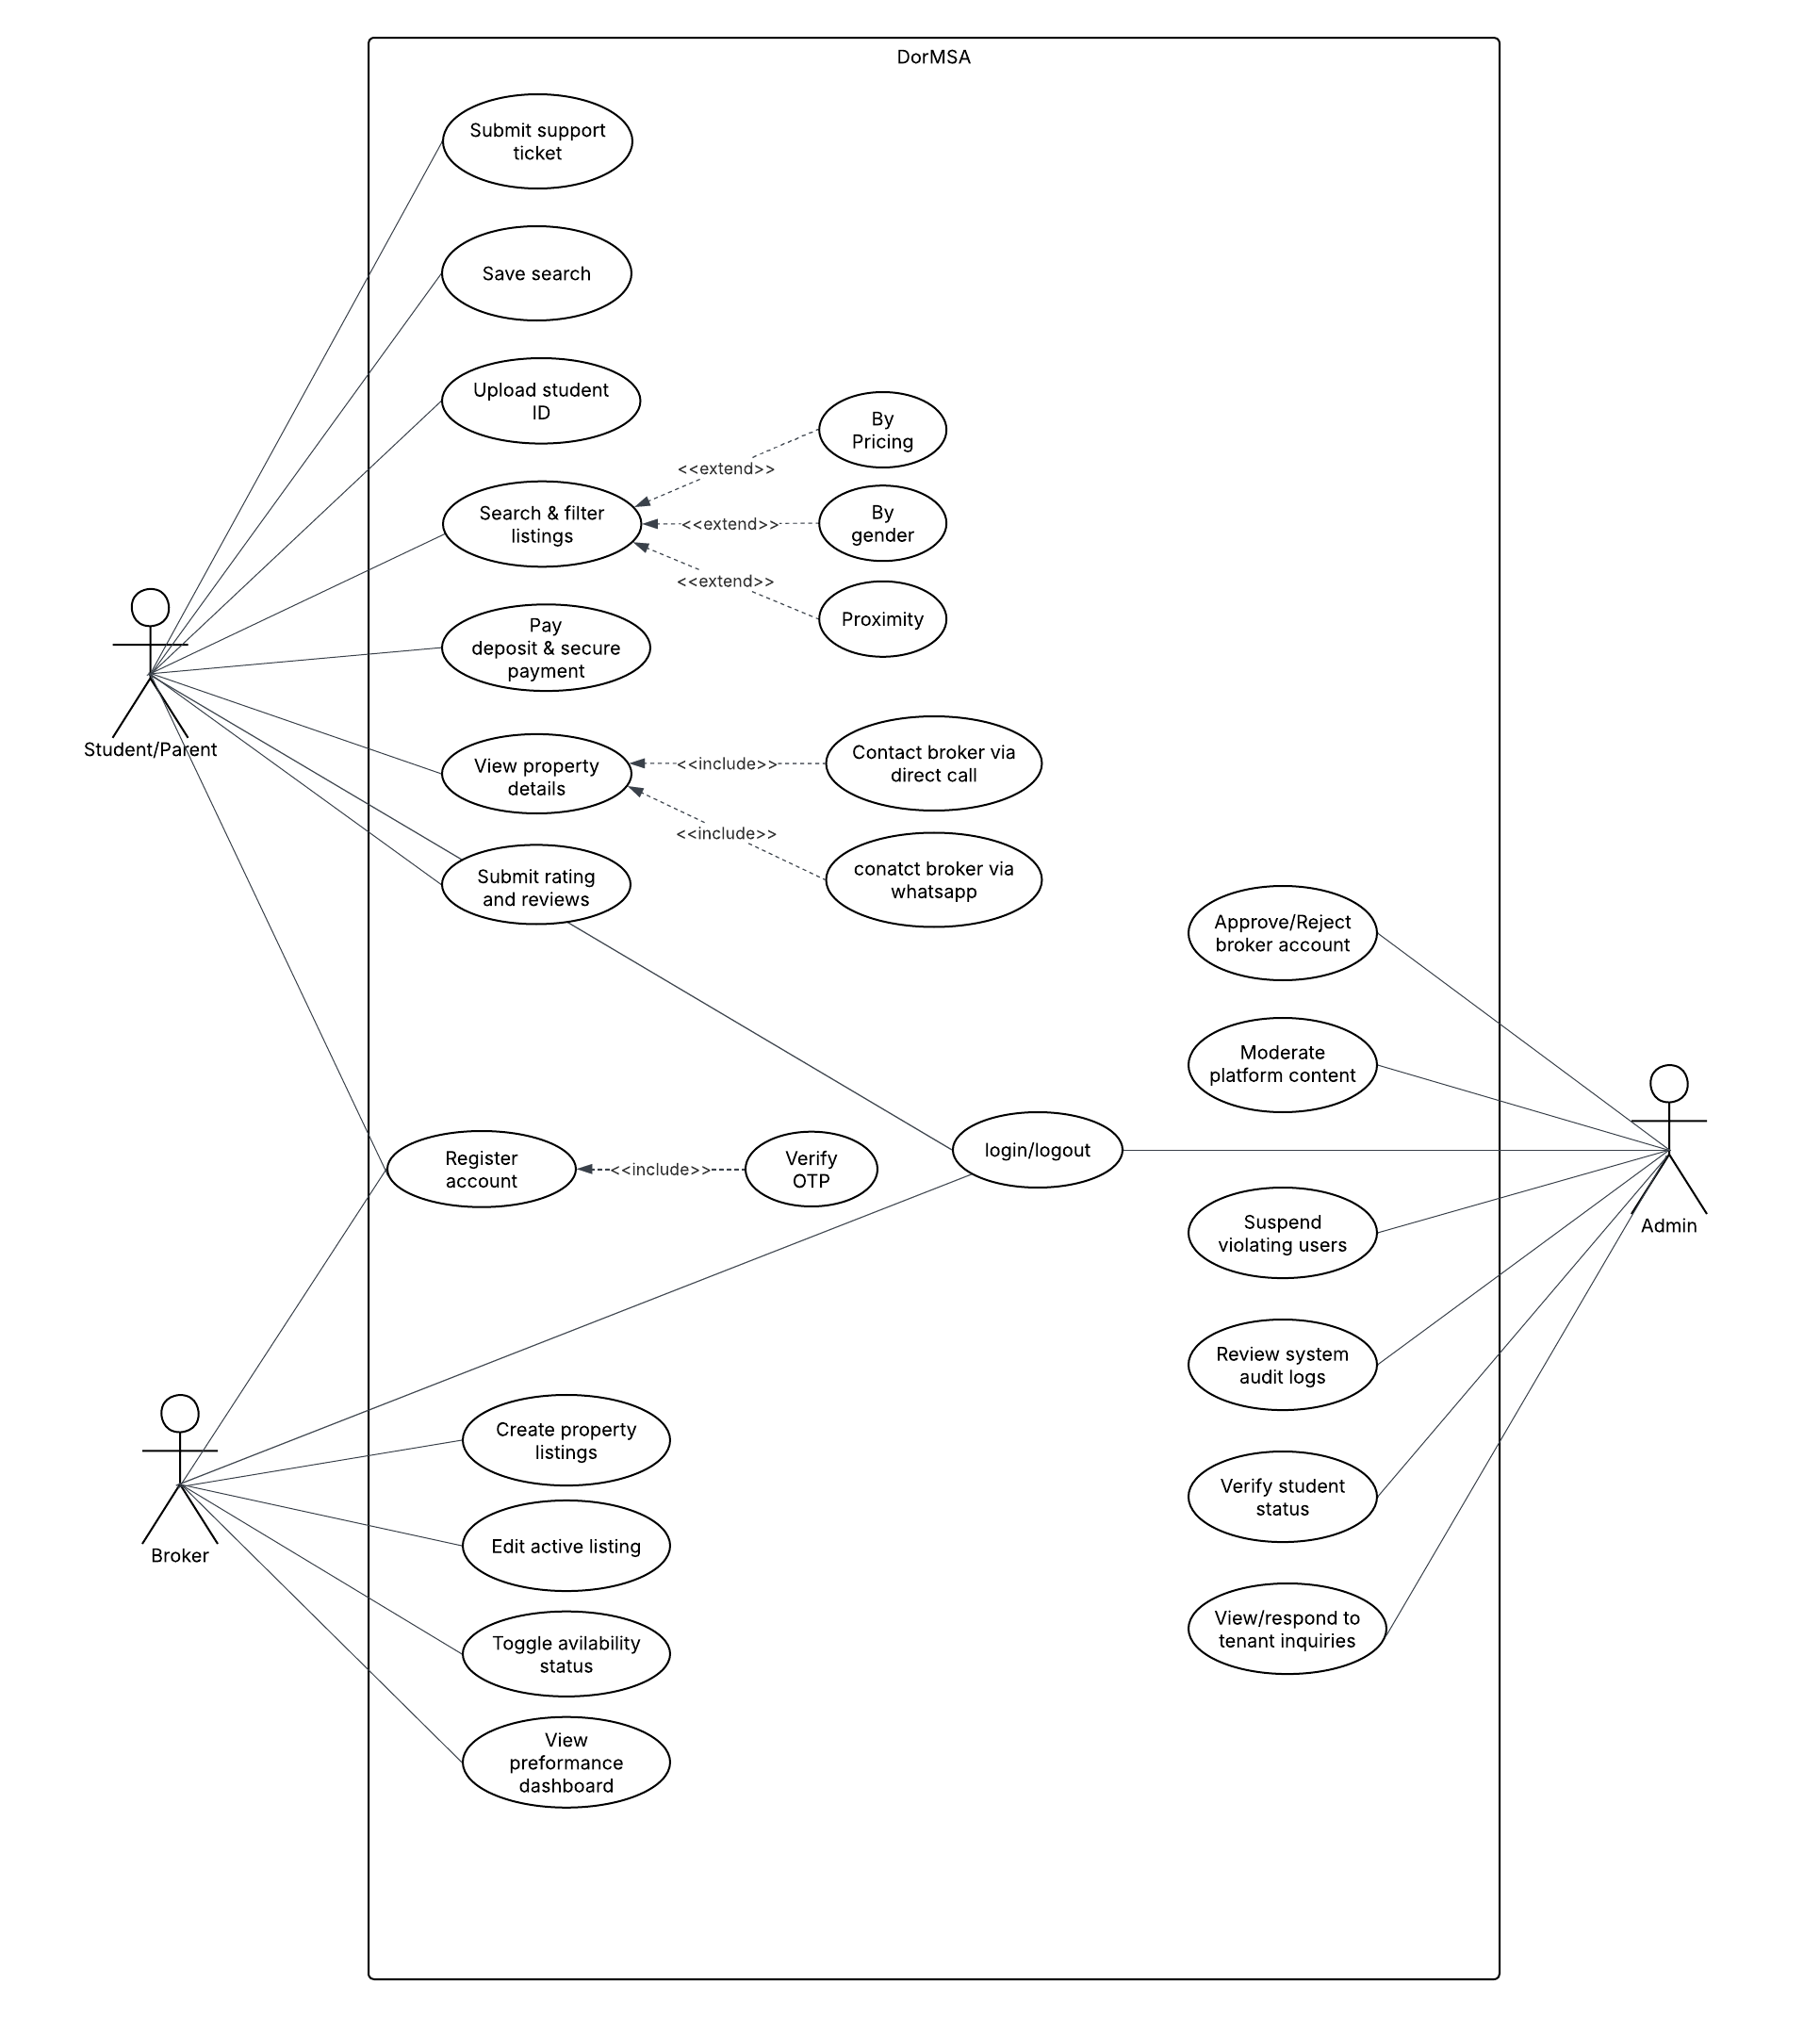
\includegraphics[width=0.9\textwidth]{DorMSA_use-case.png}
    \caption{DorMsa Use Case Diagram}
    \label{fig:usecase}
\end{figure}

\subsection{Component Diagram}
The Component Diagram details the physical structure of the components in the system and their wiring. The diagram shows the provided and required interfaces for each service component and their dependencies.

\begin{figure}[H]
    \centering
    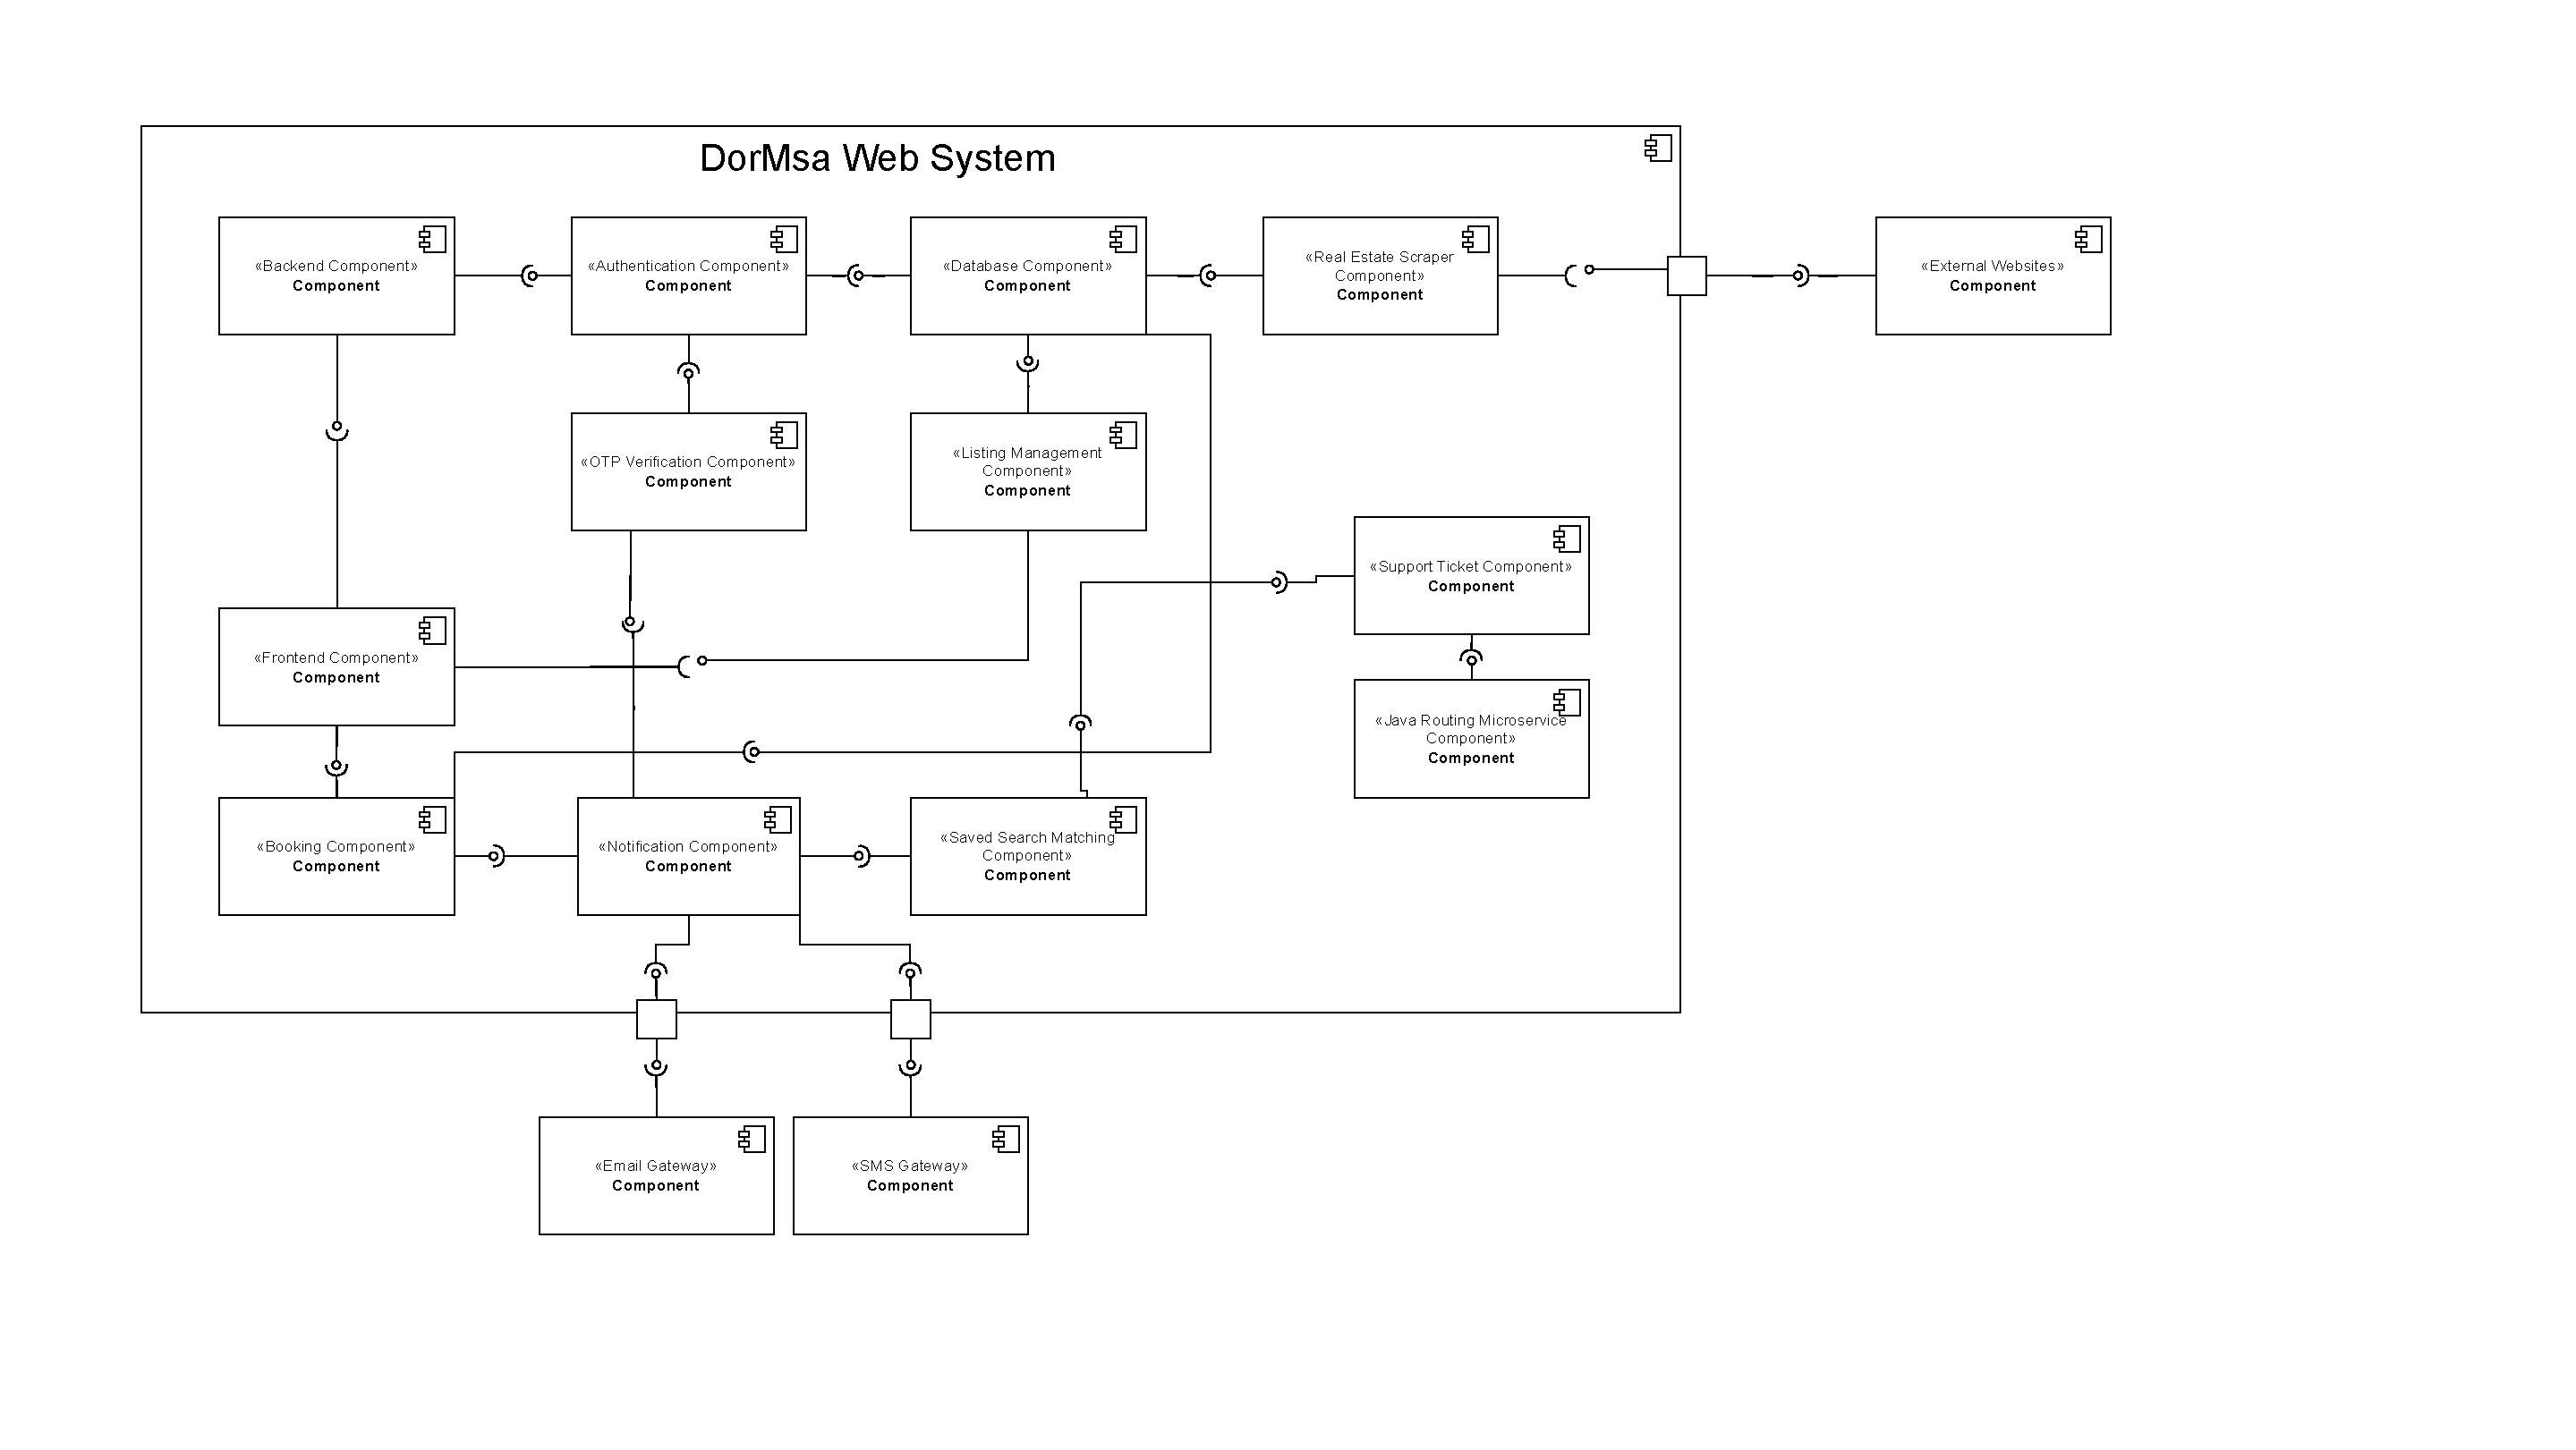
\includegraphics[width=0.95\textwidth]{Component_diagram.pdf}
    \caption{DorMsa Component Diagram}
    \label{fig:component}
\end{figure}

\newpage
\section{Overall System Design and Architecture}

\subsection{Preliminary Object-Oriented Domain Analysis}

\subsubsection{Inheritance Relationships}
User is an abstract base class. Student, Broker, and Admin are concrete subclasses that inherit common attributes and operations such as userID, name, phone, login(), and logout(), while each adds its own role-specific behaviour.

\begin{verbatim}
User (abstract)
|-- Student
|-- Broker
|-- Admin
\end{verbatim}

Additional associations: Listing is owned by Broker. Booking links Student and Listing. Review is authored by Student and references a Listing. Notification can be sent to any User.

\subsubsection{Class Descriptions}
\begin{itemize}[leftmargin=0.5cm]
    \item \textbf{User (Abstract)}: 
    \begin{itemize}
        \item \textbf{Purpose}: Base entity representing any registered platform user.
        \item \textbf{Attributes}: userID: String, name: String, phone: String (encrypted), role: Enum \{Student, Broker, Admin\}, isVerified: Boolean, sessionToken: String.
        \item \textbf{Operations}: register(), login(), logout(), editProfile(), resetPassword().
    \end{itemize}
    
    \item \textbf{Student (Concrete)}: 
    \begin{itemize}
        \item \textbf{Purpose}: Represents an MSA student or parent looking for housing.
        \item \textbf{Attributes}: studentID: String, savedSearches: \texttt{List<SearchCriteria>}, shortlist: \texttt{List<Listing>}, paymentHistory: \texttt{List<Transaction>}.
        \item \textbf{Operations}: searchListings(filters), saveListing(listing), payDeposit(listing, amount), submitReview(rating, text).
    \end{itemize}
    
    \item \textbf{Broker (Concrete)}: 
    \begin{itemize}
        \item \textbf{Purpose}: Represents a property owner or agent who manages listings.
        \item \textbf{Attributes}: brokerID: String, idDocuments: \texttt{List<File>}, isApproved: Boolean, verificationBadge: Boolean, dashboardMetrics: DashboardData.
        \item \textbf{Operations}: createListing(), editListing(listing), toggleAvailability(listing), viewDashboard(), submitIdentity(docs).
    \end{itemize}
    
    \item \textbf{Admin (Concrete)}: 
    \begin{itemize}
        \item \textbf{Purpose}: MSA staff member responsible for moderation and oversight.
        \item \textbf{Attributes}: adminID: String, permissions: \texttt{List<String>}.
        \item \textbf{Operations}: verifyBroker(broker), moderateContent(listing), suspendUser(user), viewAnalytics().
    \end{itemize}
    
    \item \textbf{Listing (Concrete)}: 
    \begin{itemize}
        \item \textbf{Purpose}: Represents a housing property posted by a verified Broker.
        \item \textbf{Attributes}: listingID: String, brokerID: String, title: String, price: Float, roomType: Enum, gender: Enum, location: GeoPoint, photos: \texttt{List<URL>}, isAvailable: Boolean, createdAt: DateTime, updatedAt: DateTime.
        \item \textbf{Operations}: publish(), hide(), flagAsDuplicate(), getDistance(campusLocation).
    \end{itemize}
    
    \item \textbf{Booking (Concrete)}: 
    \begin{itemize}
        \item \textbf{Purpose}: Represents a confirmed housing reservation between a Student and a Broker.
        \item \textbf{Attributes}: bookingID: String, studentID: String, listingID: String, depositAmount: Float, status: Enum \{Pending, Confirmed, Cancelled\}, confirmedAt: DateTime.
        \item \textbf{Operations}: confirmBooking(), cancelBooking(), generateReceipt().
    \end{itemize}
    
    \item \textbf{Review (Concrete)}: 
    \begin{itemize}
        \item \textbf{Purpose}: Stores student feedback for a listing or broker.
        \item \textbf{Attributes}: reviewID: String, authorID: String, targetID: String, rating: Integer (1--5), text: String, createdAt: DateTime.
        \item \textbf{Operations}: submit(), publish(), delete().
    \end{itemize}
    
    \item \textbf{Notification (Concrete)}: 
    \begin{itemize}
        \item \textbf{Purpose}: System-generated message dispatched to users on trigger events.
        \item \textbf{Attributes}: notifID: String, recipientID: String, type: Enum \{Booking, Expiry, NewListing\}, channel: Enum \{SMS, Push, Email\}, deliveredAt: DateTime.
        \item \textbf{Operations}: send(), retry(), markDelivered().
    \end{itemize}
\end{itemize}

\subsection{Microservice Component-Based Architecture}
Each component configured in the system adheres to Component-Based Programming (CBP) principles of provided and required interfaces under an Inversion of Control (IoC) framework.

\begin{table}[H]
\centering
\small
\renewcommand{\arraystretch}{1.3}
\begin{tabular}{p{0.04\textwidth} p{0.28\textwidth} p{0.28\textwidth} p{0.34\textwidth}}
\toprule
\textbf{\#} & \textbf{Provided Interface} & \textbf{Concrete Class} & \textbf{Description} \\
\midrule
1 & \hspace{0pt}Email\-Gateway & \hspace{0pt}Mock\-Email\-Gateway & Development gateway logging email contents to the terminal. \\
2 & \hspace{0pt}Email\-Gateway & \hspace{0pt}Smtp\-Email\-Gateway & Simulates connection to institutional SMTP server. \\
3 & \hspace{0pt}Notification\-Service & \hspace{0pt}Console\-Notification\-Service & Handles user alerts and delegates delivery to email port. Required: \hspace{0pt}Email\-Gateway, \hspace{0pt}Message\-Store\-Service. \\
4 & \hspace{0pt}Support\-Router\-Service & \hspace{0pt}Simple\-Support\-Router\-Service & Automates support helpdesk routing assignments. Required: \hspace{0pt}Notification\-Service, \hspace{0pt}Message\-Store\-Service. \\
5 & \hspace{0pt}Saved\-Search\-Matcher\-Service & \hspace{0pt}Simple\-Saved\-Search\-Matcher\-Service & Matches property uploads against user searches. Required: \hspace{0pt}Notification\-Service. \\
6 & \hspace{0pt}Message\-Store\-Service & \hspace{0pt}Simple\-Message\-Store\-Service & Normalizes phone numbers and logs OTPs/system events. \\
\bottomrule
\end{tabular}
\caption{System Component Directory}
\label{tab:components}
\end{table}

\newpage
\section{Screenshots for the User Interface}
The following screenshot illustrates the live application interface: the left-hand panel shows the student dashboard (including active OTP phone number validation banners and status indicators), while the right-hand panel shows the real-time Java microservice dashboard logging autowired components, verification transactions, and support ticket assignments.

\begin{figure}[H]
    \centering
    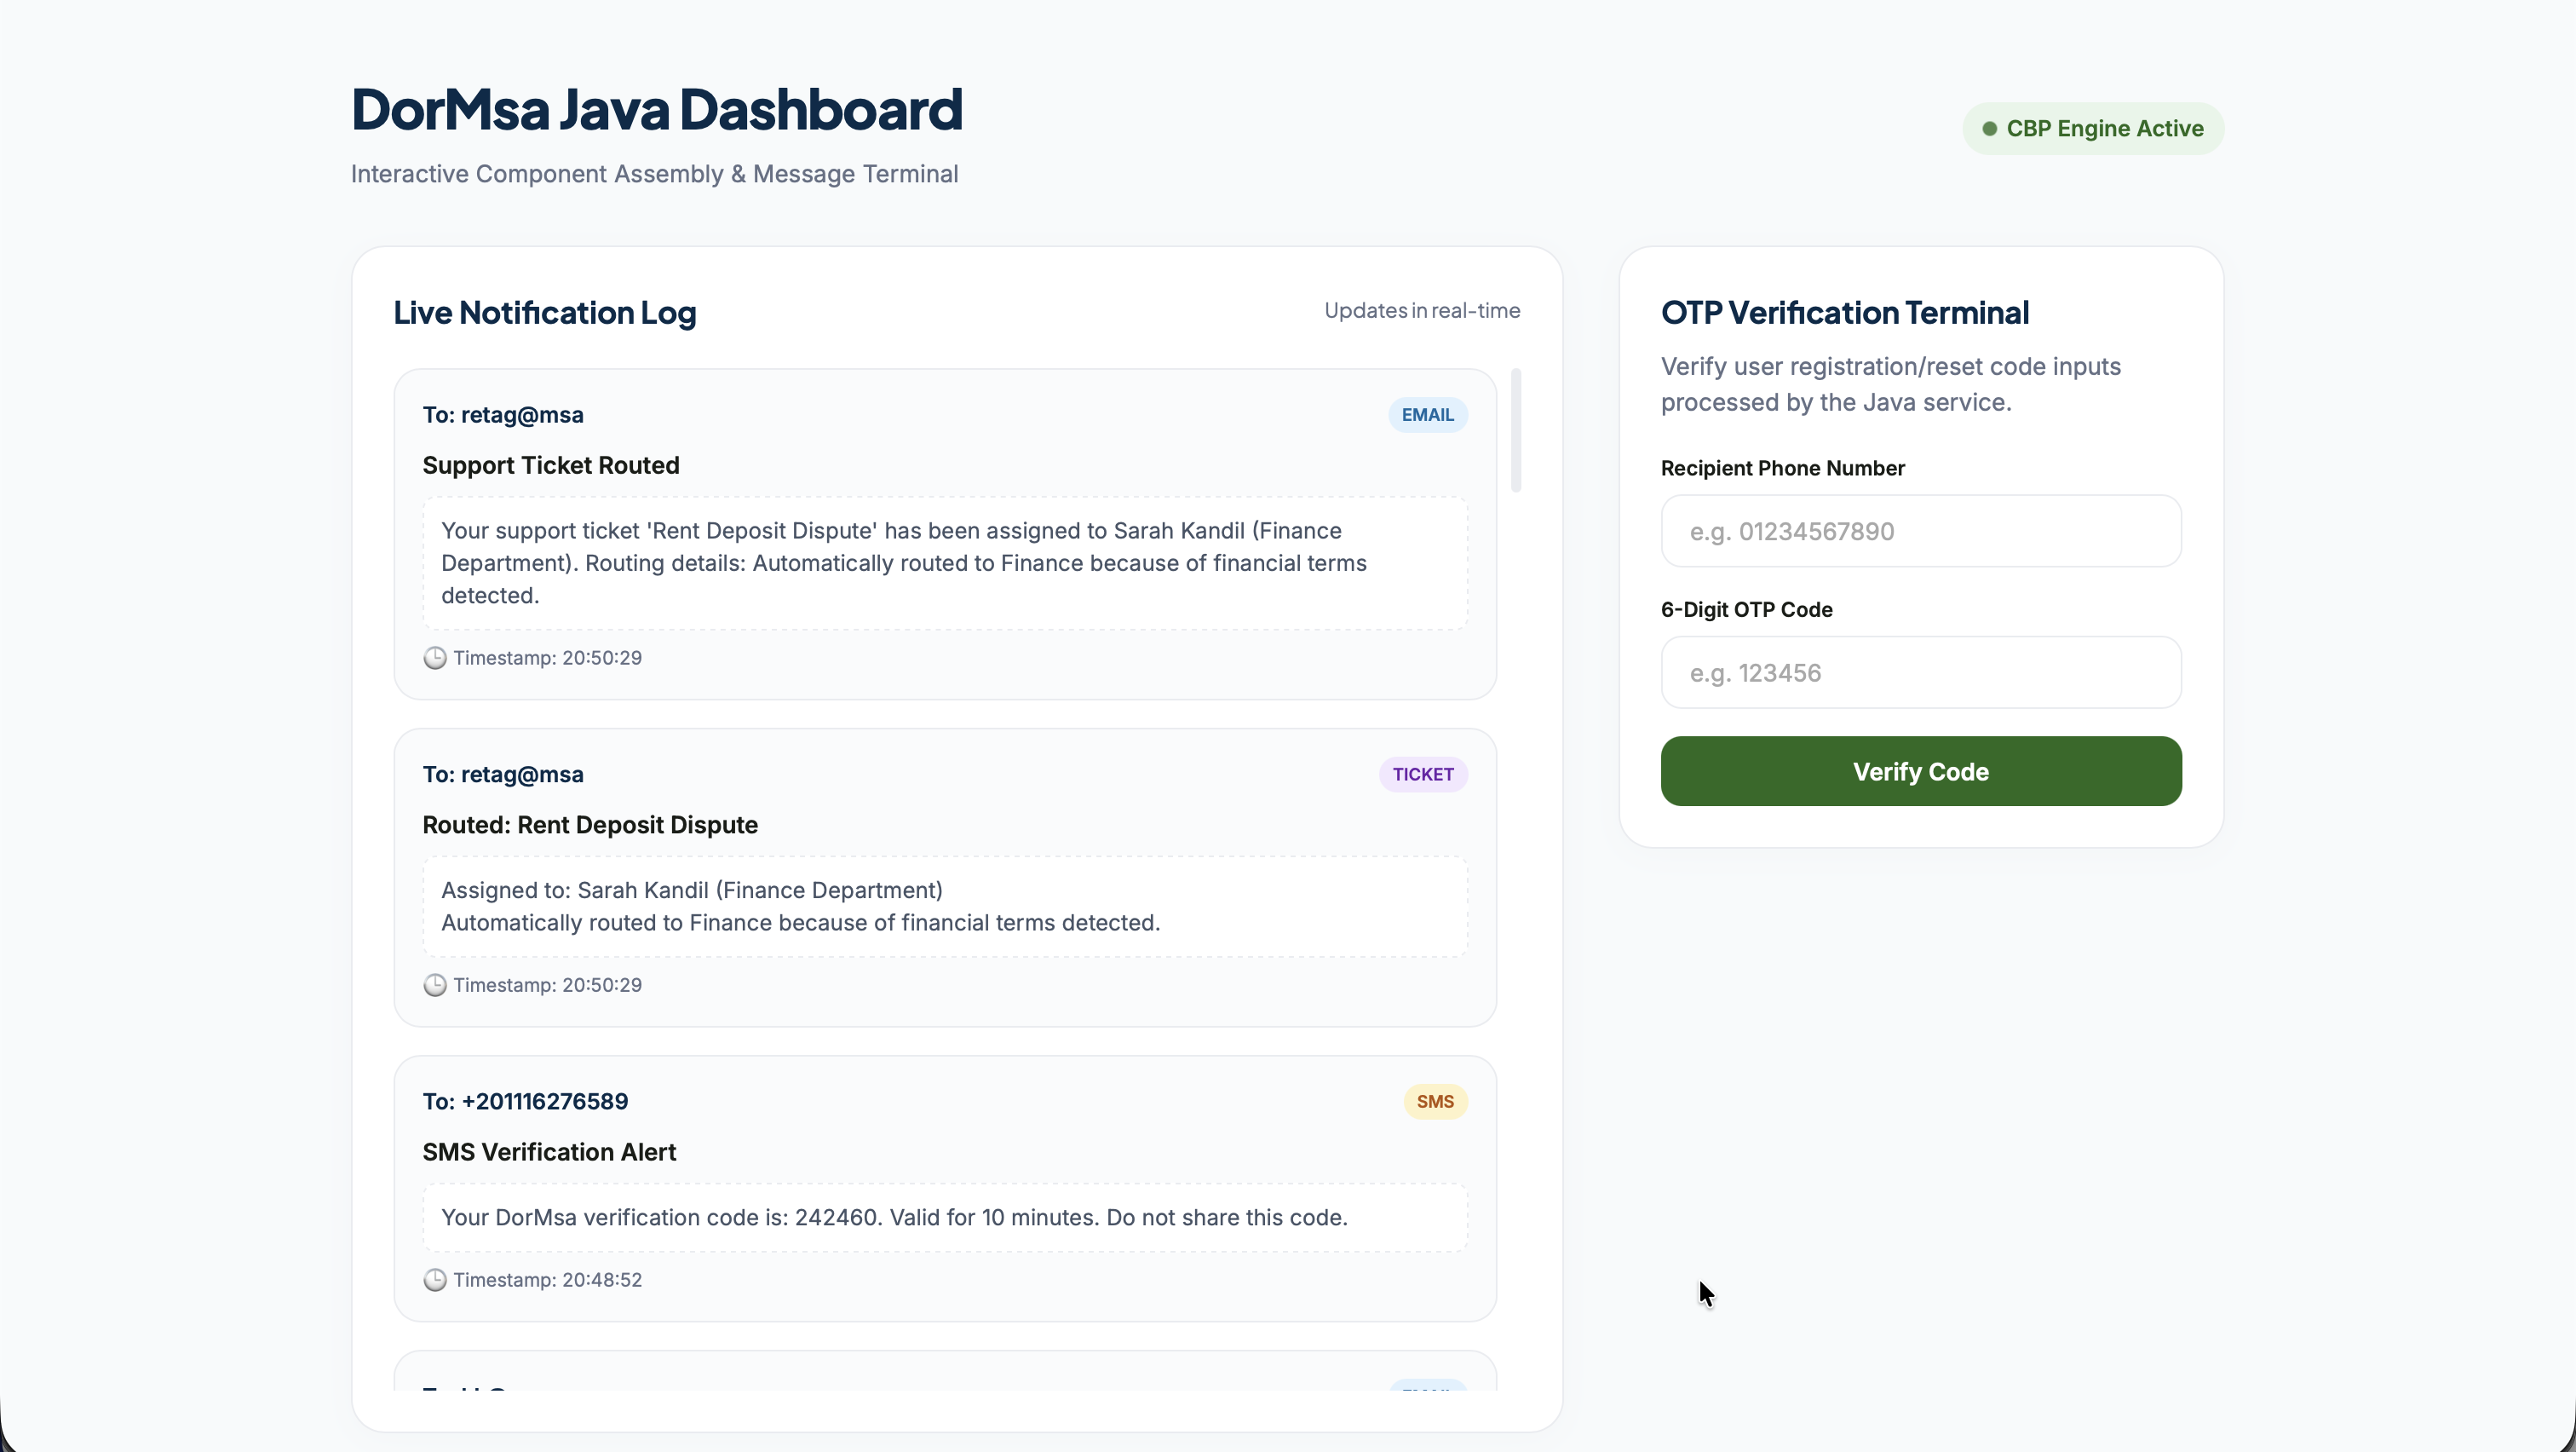
\includegraphics[width=\textwidth]{ui_screenshot.png}
    \caption{DorMsa User Interface - Dashboard and Java Component Logs}
    \label{fig:uiscreenshot}
\end{figure}

\end{document}
